\section{\plink: Discovering and Exploiting Datacenter Network Locality for Efficient Cloud-based Distributed Training}

So far we have focused on accelerating distributed learning at a rack scale, by customizing hardware configuration, software stack, and network interconnect. While highly effective, not all of the optimizations are universally applicable, for example, in a public cloud environment. Further, even if all optimizations are applied, they do little to address cloud specific bottlenecks.

\subsection{Specific Challenges in Public Clouds}
Two major challenges exist in cloud-based training.

\noindent\textbf{Non-uniform link bandwidth}. Host-to-host bandwidth in the cloud is non-uniform due to the hierarchical structure of the datacenter~(\textsection \ref{sec:datacenternetwork}). %, as VM nodes can be spread across different physical hosts, racks, rows or even clusters. %Practically, VMs can spread in multiple physical machines, racks, rows, or even clusters. If the network core utilization is high, or the oversubscription ratio is large, available bandwidth for a pair of VM flow will be smaller when compared to intra-rack traffic (section \ref{sec:datacenternetwork}). Achieving consistent high performance requires minimized cross rack traffic. 
Figure \ref{fig:dcnetworkcondition} shows a pairwise bandwidth probe of 32 VM nodes in \ectwo and \azure, in the same availability zone/datacenter. In both cases, faster pairs can deliver more than 2x the throughput of slower pairs. % during \code{iperf} probes.%, when running point to point iperf probe. 

%The nodes appear to form two clusters with intra-cluster communication delivers almost 2x the performance of inter-cluster communication. 

\noindent\textbf{Volatile traffic}. The performance variability in the public cloud is well known~\cite{cloudVariance1, Iosup:2011:PVP:2007336.2007402,perfVariance}. Although mechanisms for performance isolation have been proposed~\cite{Shieh:2010:SPI:1863103.1863104,Shieh:2011:SDC:1972457.1972489}, we still observe interference from other workloads, leading to volatile latency and aggregation performance (Figure~\ref{fig:perfFluctuation}).
%\arvind{we don't provide experimental evidence; so reword to make it clear.  maybe say something like "we observed ...".}

%Although multiple previous work~\cite{Shieh:2010:SPI:1863103.1863104,Shieh:2011:SDC:1972457.1972489} has purposed mechanisms for performance isolation, empirically we can still observe interference by other workloads. Figure \ref{fig:dcnetworkcondition} (Right) traces the 10-second bandwidth average of two VMs for 90 minutes on Azure US-West region. The bandwidth can vary from 10 to 20Gbps. As a result, the significant changes in link condition infers that the best aggregation route is not static. 

\begin{figure}[t!]
	\centering
	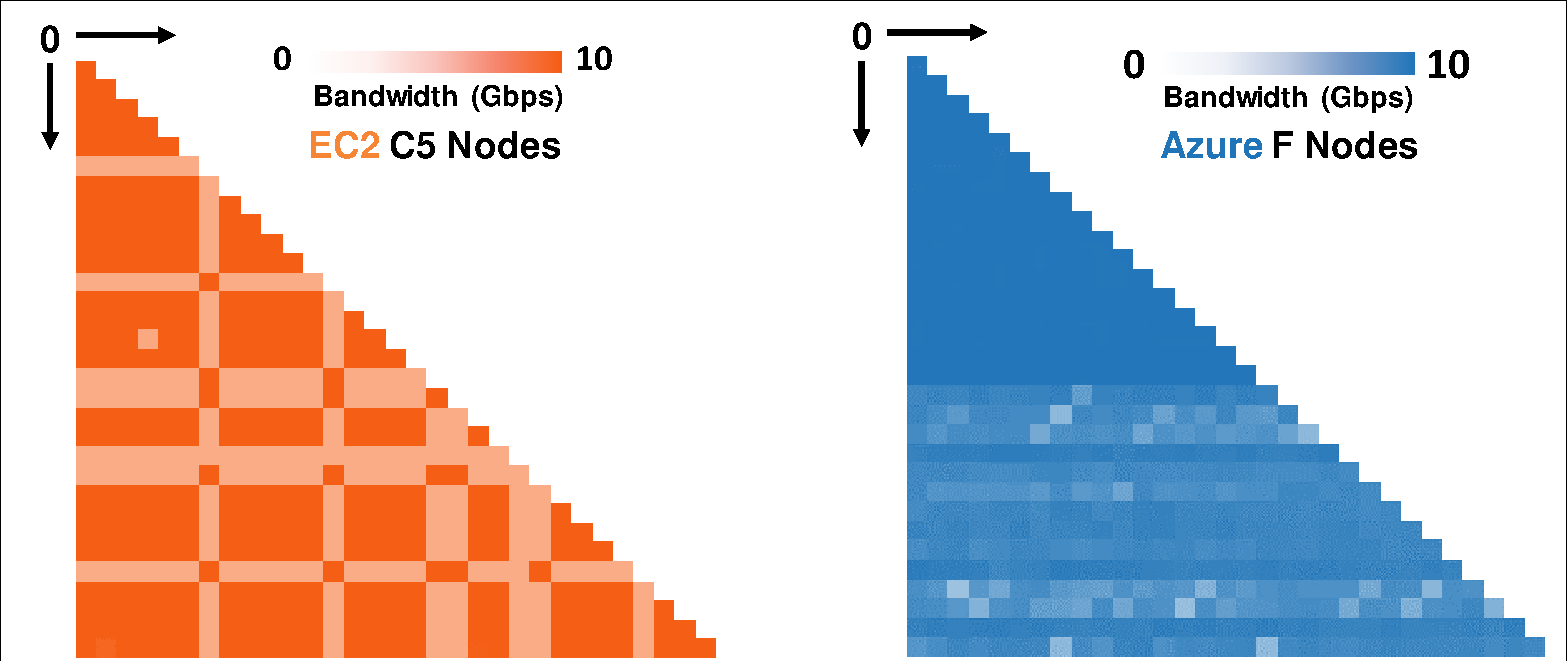
\includegraphics[width=.7\linewidth, trim=3 3 3 3,clip]{Figures/dcnetworkcondition.pdf}
	\caption{Pairwise bandwidth probes with 32 \ectwo C5 and \azure F instances show non-uniform link bandwidth.}
	\label{fig:dcnetworkcondition}
\end{figure}

\begin{figure}[t!]
	\centering
	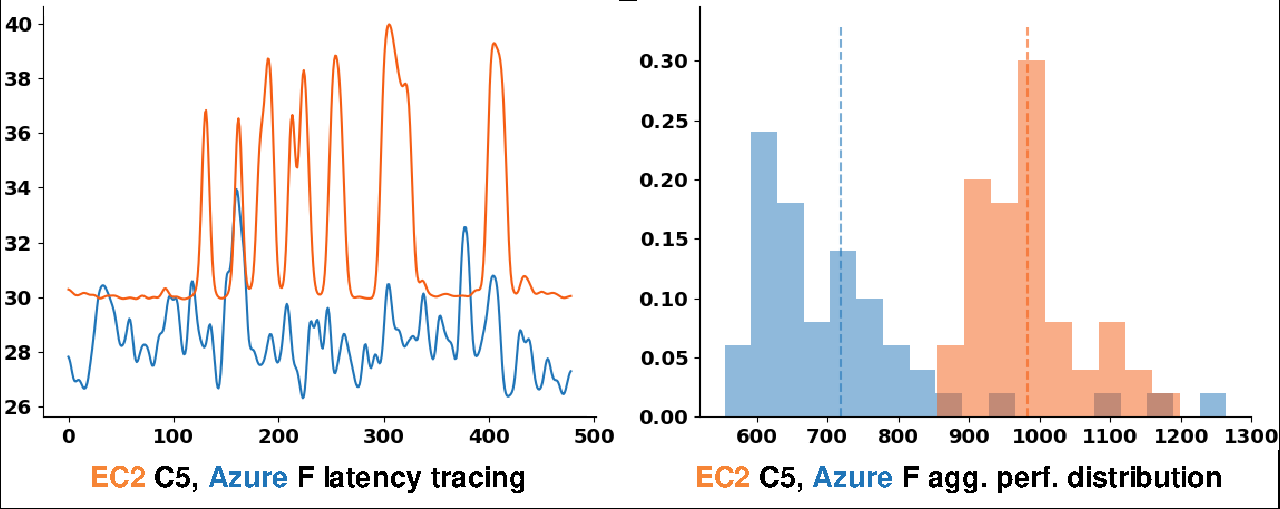
\includegraphics[width=.7\linewidth, trim=3 3 3 3,clip]{Figures/perfFluctuation.pdf}
	\caption{Left: 8 hour latency (us) tracing (1 minute average) between two VMs on both clouds show steep latency fluctuations due to volatile cloud traffic. Right: Wide performance distribution of the same, periodically launched Gloo aggregation task on both clouds.}
	\label{fig:perfFluctuation}
\end{figure}

%\noindent\textbf{One route does not fit all}. The size of model of different layer in a neural network can vary significantly (e.g., the size of the largest layers in the popular ResNet-50 model is multi-megabytes in Caffe2 versus a small layer's model size of hundreds of bytes). This means the transmission time of some layers is latency-bound while some are bandwidth bound. Since the forward and backward passes process layers in a fixed order, a delay in the update of layer L will cause process stall of layer L+1 in forward pass or L-1 in backward pass. Therefore, optimally hiding communication latency requires different aggregation routes for different layers.

\subsubsection{Inefficiencies in Existing Approaches}
\label{sec:differentReductionAlgorithms}
We motivate our design by analyzing why some existing approaches do not perform optimally, as they rely on assumptions that aren't typically valid in the datacenter setting. 

%We first define good locality as localizing communication within a single rack. Thus, the more cross rack communication, the worse locality.

\begin{figure}[t!]
	\centering
	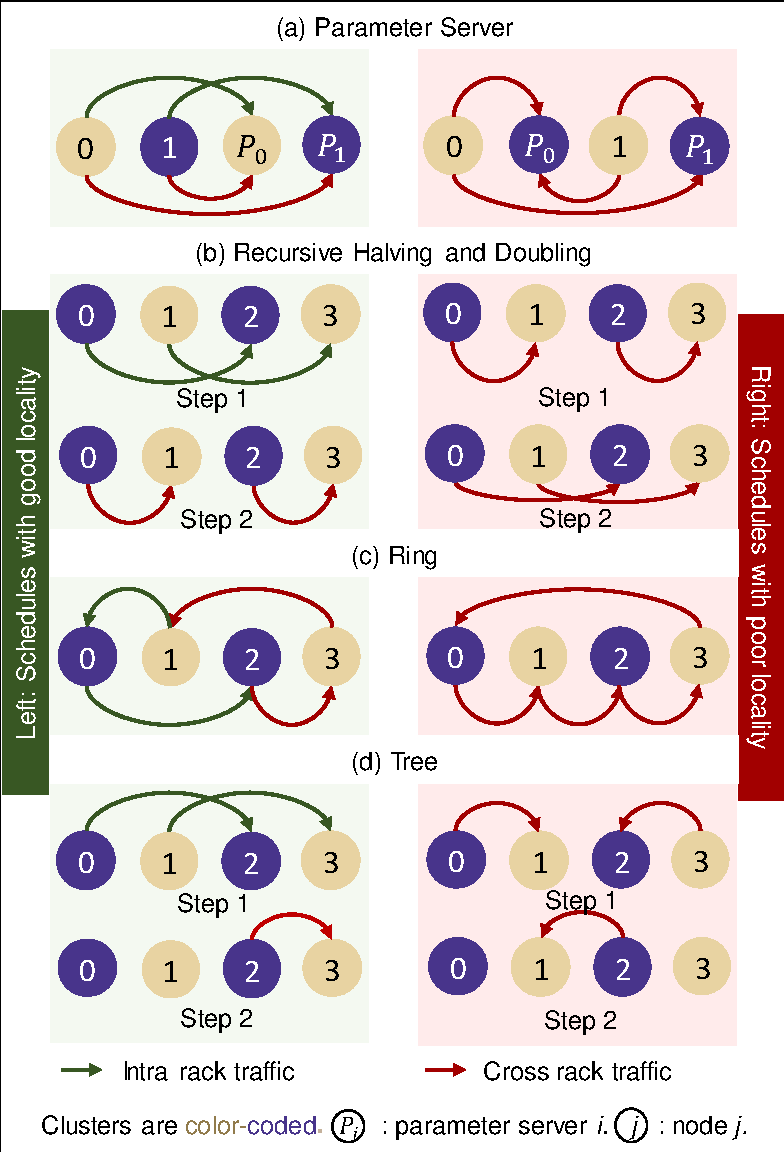
\includegraphics[width=.5\linewidth, trim=3 3 3 3,clip]{Figures/poorlocalitywithexistingapproach.pdf}
	\caption{Existing aggregation approaches can suffer from poor locality if not taking physical network topology into account.} %Some steps omitted for clarity.}
	\label{fig:poorlocalitywithexistingapproach}
\end{figure}

Figure \ref{fig:poorlocalitywithexistingapproach} shows a theoretical analysis of widely used communication patterns. PS (a) and popular choices of CA such as halving-doubling (b) and ring (c) are shown in a setup where nodes (0-3, enclosed in a circle) are spread equally among two clusters (purple and gold).  The left side of the figure shows patterns that achieve optimal locality in the setting by exchanging data among nodes with high locality (high-performance links in green) while minimizing transfers over the bottleneck links (slow links in red). The right side shows alternative reduction routes with poor locality. All patterns achieve the same result, but with different efficiency.

The problem with poor locality happens when the communication pattern in the algorithm is not optimally aligned with physical topology. Mapping logical ranks to physical hosts in a locality-preserving way is contingent on awareness of the physical network structure. Hence, \textit{topology-awareness} is crucial for efficient aggregation in a datacenter network. %For example, in the case of the bad recursive halving-doubling communication highlighted in Figure \ref{fig:poorlocalitywithexistingapproach}(b-right), it would be much better if the IDs of node 1 and 2 are swapped, creating the pattern on the left. %
%Being able to do so 

Even with careful mapping, not all algorithms work optimally in the datacenter environment. Table \ref{table:algoCharacterization} summarizes network characteristics of these algorithms, with a simplified, flattened datacenter network topology model where nodes are simply placed in different racks. Centralized PSs are known to suffer from \textit{incast} congestion and do not scale to a large number of workers~\cite{firecaffe,Geng:2018:HHP:3229543.3229544}. Sharded PSs incur high cross rack traffic. CAs usually trade off lower per-link traffic on the wire with more rounds of communication, which is not suitable when the latency is high. Tree reduction inherits the problems of both PS and CA: high fan-out causes incast problems; a low fan-out adds more rounds. Ultimately, we need an algorithm that bounds communication steps, takes advantage of fast links, and localizes traffic to avoid interference from competing traffic.

\begin{table}[ht]
	\centering
	\begin{tabular}{|c|c|c|c|}
		\hline 
		Name & Rounds/Hops & Bytes on Wire & XR Bytes \\
		\hline
		PS (fully sharded)  & $2$ & $2(NC-1)S$ & $2N(C-1)S$  \\
		\hline
		Halving doubling & $2log_2NC$ & $2NCS$ & $2C\frac{N-1}{N}S$ \\ 
		\hline 
		Ring-Chunked & $2NC-1$ & $(2NC-1)S$ & $(2C-1)S$ \\
		\hline
        Tree (fan out = C) & $2(log_CN + 1)$ & $\approx2C\frac{CN-1}{C-1}S $ & $\approx2C\frac{(N-1)}{C-1}S$ \\ %n is a power of k. each k link starting from the 2nd layer, at least k-1/k links are cross machine link
        \hline
        \hline
        2-level hierarchical & $4$ & $2S(NC-1)$ & $2(C-1)S$ \\
		\hline
	\end{tabular}
	\caption{Network characteristics of various algorithms featuring rounds of communication (Rounds), minimum total traffic (Bytes on Wire), and minimum cross rack traffic (Min XR Bytes, corresponding to red arrows in Figure~\ref{fig:poorlocalitywithexistingapproach}) to allreduce with $NC$ nodes on $C$ racks, each with $N$ nodes. Each node has a buffer of size $S$ bytes. PS and aggregators in HA are colocated and sharded.}
	\label{table:algoCharacterization}
\end{table}

\subsubsection{2-level Hierarchical Aggregation (2LHA)}
HA is not new, but most applications of \mlha are in contexts where the network topology is known. HA does not reduce the total amount of data transferred on the wire, but it can create more \textit{localized} traffic and avoid slow links.

%trades more \textit{localized} traffic with higher \textit{latency}, because a piece of data needs to traverse multiple hops.

%The potential benefit comes from traffic localization, which is related to the tree-like topology: with each hop the message takes, exponentially more machines can generate adversarial traffic that affects this message.
One important parameter in HA is the number of levels. Similar to~\cite{cool}, we used a 2-level HA based on our domain knowledge of datacenter networks, that oversubscription mostly hurts at the rack level. Thus, by separating inter- and intra-rack aggregation, we can best capture the static aspect of locality and minimize latency. The use of more levels ($>2$) suffers from higher latency and volatile performance, as messages need to traverse multiple links with unpredictable latency, but provides no benefit compared to PS if links don't have enough non-uniformity (e.g., in the same cluster). %Therefore, we focus on a 2-level hierarchical (2LHA) aggregation scheme because it strikes a balance between smaller latency (requiring fewer rounds) and more aggressive localization (requiring more rounds).

%, and empirically can capture the network locality well~(\textsection\ref{sec:eval}).

\label{sec:2lhaOverview}
\mlha partitions nodes into different groups (clusters) based on their affinity. \mlha starts by chunking the buffer across members in the same group. For each chunk, a node is designated as the local master (LM) for that group for aggregating locally. One of the LMs across all groups is chosen as the global master (GM) for global aggregation. Visually, the reduction trees of all chunks form a 2-level forest. Communication for \mlha is done in the following steps: 

\begin{enumerate}[noitemsep,topsep=0pt,parsep=0pt,partopsep=0pt]
  \item Each group member sends all chunks to their respective LMs (intra-group traffic only).
  \item LMs in all groups send per-group aggregated chunk to the GM for global aggregation (inter-group traffic only).
  \item The GM aggregates the chunk, then uses the reversed routes for propagating the globally-aggregated chunk back to the LMs.
  \item The LMs fan out the globally aggregated chunk to all group members.
\end{enumerate}

%\arvind{say something about sharding and load balancing of chunks?}

%\begin{figure}
%	\centering
%	\includegraphics[width=.9\linewidth, trim=1 3 3 3,clip]{Figures/2LHA.pdf}
%	\caption{The first two steps in performing a \mlha for chunk 1 labelled. Gradients are aggregated locally before synchronized globally, reducing data transferred on inter-group links.}
%	\label{fig:2lha}
%\end{figure}

\mlha is described here as a two-phase process for simplicity, but the intra- and inter-group aggregation can overlap. Effective \mlha also requires load-balanced LM and GM assignments within and across groups. Later we provide an implementation that satisfies these. Table \ref{table:algoCharacterization} shows the desirable properties of \mlha. Compared to CAs, the number of rounds in \mlha does not increase with the number of nodes and, compared to PSs, it requires significantly less cross-rack bandwidth.

\subsection{Design and Implementation of \plink}

We now describe \plink, an optimized, topology-aware, and dynamic system that leverages HA for efficient cloud-based training. To optimally utilize datacenter networks, \plink must address the major challenges highlighted previously. \plink uses three components to achieve this.
\begin{itemize}[noitemsep,topsep=0pt,parsep=0pt,partopsep=0pt,leftmargin=1em]
    \item \marcopolo: a network probing and clustering approach to capture physical locality in the datacenter network. \marcopolo groups nodes based on their physical affinity, so intra-group links have better communication performance than inter-group links. %\arvind{say "better communication performance" rather than "lower latency"?}
    \item \ha: a high-performance implementation of \mlha that is codesigned to take advantage of deep learning properties. %\arvind{what do you mean by training workload?}
    \ha uses clustering information to  distribute the aggregation workload efficiently and execute the aggregation schedule.
    \item \autoplink: a mechanism that tracks training performance and adjusts the current GM and LM assignments to adapt to changes in the network conditions.
\end{itemize}

\subsubsection{Capturing Network Locality with \marcopolo}
\label{sec:marcopolo}
For accurate network topology discovery, \marcopolo must probe quickly and should not rely on knowledge of a particular datacenter. \marcopolo: (1) probes communication links between nodes to measure pairwise node distances, (2) denoises probed distances, and (3) clusters nodes.

\paragraph{Running \marcopolo probes}

\marcopolo starts by issuing measurements to identify communication locality and determine pairwise node distances. Distance is defined using universal networking concepts, like latency or inverse bandwidth. \marcopolo uses two different probes: an inhouse DPDK-based~\cite{HomeDPDK74:online} probe to provide near bare-metal latency measurements for supported VMs on \azure and \ectwo, and iPerf~\cite{iPerfThe0:online}. \marcopolo runs these networking probes one-to-one. $O(N^2)$ time would be required to probe $N$ nodes if run sequentially. To accelerate this process, \marcopolo picks as many pairs (up to $\frac{N}{2}$) as possible in each round without having a node appear twice, to avoid interference from concurrent tests. This allows \marcopolo to probe in $O(N)$ rounds.

%\noindent\textbf{All-to-all probes} are one-shot tests that all nodes participate in. \marcopolo use these tests to assess distances of nodes in a more dynamic fashion under loaded conditions. %, as all to all probe resembles the communication pattern of distributed training. 

\marcopolo derives pairwise distances with probe results (in case of bandwidth measurements, bandwidth are converted to distance by taking the inverse~\cite{affinity2Distance}). \marcopolo then proceeds to \textit{denoise} the collected data. %, before clustering nodes into different groups based on their physical affinity. %\arvind{be consistent with terminology.  Earlier it is "augment/denoising", now it is "augment", and next it is "refining".  I think "denoising" is better.}

\paragraph{Denoising probe data with embedding}
\label{sec:embedding}
 \marcopolo embeds nodes in a Euclidean coordinate space, obtaining a set of coordinates whose distances agree with the probed distances. This works to:
\begin{enumerate}[noitemsep,topsep=0pt,parsep=0pt,partopsep=0pt]
    \item Denoise measurements by leveraging Euclidean space to approximate the physical location of nodes. %\arvind{I think we can say "which we use to approximate the physical location of nodes inside a datacenter" rather than "resembles a network topology".}
    %Distances in the Euclidean space end up being more reflective of network topology, likely due to denoising effects.
    \item Obtain a set of ``virtual coordinates'' for a clustering algorithm to identify groups.
\end{enumerate}
To embed nodes, we identify node coordinates ($\mathbf{v_i}$ and optional $h_i$) that minimize the following objective:
\begin{equation}
    \sum_{i=1}^n \sum_{j=1}^{i-1} \left( (d_{i,j})^\alpha + \mathbbm{1}_h\left[h_i + h_j \right]  - p_{i,j}\right)^2 
\end{equation}
where $n$ is the number of nodes, $d_{i,j} = \left\lVert \mathbf{v_i} - \mathbf{v_j} \right\rVert_2$ is the Euclidean distance between embedded node coordinates for nodes $i$ and $j$, $p_{i,j}$ is their probed distance, parameter $\alpha$ takes a value between 1 and 2, $h_i$ is a non-negative startup cost parameter for node i, and $\mathbbm{1}_h$ is a switch for $h_i$. We use the Adam algorithm~\cite{kingma2014adam} to optimize this.
%$x$ is a tunable parameter between 1 and 2 that intuitively governs how much emphasis is put on long probed distances in the embedding process. %is an indicator denoting whether or not we are using these latency parameters. % We will describe the use of $h_i$ later in this section, but first consider the case when $\mathbbm{1}_h = 0$.

\marcopolo embeds VM nodes in a coordinate space that preserves the probed distances between VM nodes. The denoising effect of the embedding process stems from its tendency to keep mutually close nodes together, which enforces our domain knowledge that VM nodes that are close to one particular reference VM node are probably close to each other as well in the datacenter. Thus, this effect has a correcting influence when the mutual-closeness property is violated by a particular observation but is observed in a majority of nodes. A lower number of embedding dimensions strengthens this effect.
%Considering only the left size of equation 1 (ignoring $h$), there are 2 cases, one when $x=1$ and one when $x=2$ (the two allowed values). These share a common intuition for why topology might be well captured. In both, we are embedding our nodes in a coordinate space where larger Euclidean distance should correspond to larger probe distance. In such a space, we have the property that, for nodes A, B, and C, if A and B are both close to C by Euclidean distance, they must also be relatively close to each other. This fits our domain knowledge, that if two nodes are close to a mutual third in a datacenter, they should also be relatively close to one another. 
%We have observed noise in the probe distance data that violates this mutual-closeness property, and we believe this is part of why our method is successful. Fitting Euclidean distance enforces this concept of closeness, working to remove that noise, and giving us refined distance with an improved agreement with true topology.

$\alpha$ tunes how longer distances are treated in the Euclidean space: $\alpha=1$ fits the embedded distances to probe distances exactly. For $\alpha>1$, we can achieve increased compaction of distance while maintaining relative distance order. This effect is desired because small physical distances can be magnified disproportionately in the probe due to competing traffic. Setting $\alpha=2$ causes the long probed values to be ``compacted'' more than the smaller ones (but it never changes the relative order of distances). Figure~\ref{fig:legacy_why} suggests empirically, a larger $\alpha$ pushes VM nodes with short distances even closer on the embedded plane, leading to more consistent clusters with higher adjusted mutual information~\cite{vinh2010information} (0.59 vs 0.76) across 100 runs.

% with a larger probe distance being represented by a moderately larger embedding distance, allowing \marcopolo to generate more consistent clusters empirically (higher Adjusted Mutual Information~\cite{vinh2010information} score across many runs).

%It is important to capture long distances as accurately as possible because they are the bottleneck in \mlha. Setting $\alpha > 1$ lets \marcopolo{} focus more on the representation of long distances in the embedding process. Figure~\ref{fig:legacy_why} (right) shows that in the $\alpha=1$ case, the error for deviating from the optimal value of embedding distance ($d$) is independent of probe value $p$, but with $\alpha > 1$, the same deviation for a longer probed distance results in a larger error in the optimization objective, forcing the optimizer to focus on it. %Setting $\alpha > 1$ does exactly this for longer probe distances, which we expect to be more important.


% we're effectively discounting long probe distance in the embedding: only 2X euclidean distance is required to represent a 4X probe distance. Preventing long distances in the embedded space enforces the reality in the datacenter that no distances should be significantly larger than the average distance, so disallowing long distances to be embedded exceedingly far from other nodes in face of a long probed distance (likely due to interference) tends to better capture physical affinity.

%$x$ also controls whether additional focus is given to long distances when minimizing the embedding error: a larger $x$ forces the embedding space to reflect long distances most precisely, which is desirable because \mlha{}'s performance is bottlenecked by the longest distance in each hierarchy. Capturing this is crucial in later generation of the actual clusters. Figure~\ref{fig:legacy_why} gives a visual summary of the effect of $x$: long probed distances are more ''compressed``, and more ''carefully treated`` than short probe distances, resulting in tighter-packed embedded space that resembles datacenter, especially bottlenecks.

Inspired by~\cite{Dabek:2004:VDN:1030194.1015471}, \marcopolo includes an optional parameter $h_i$, the node-specific, network-agnostic, fixed latency of sending a packet (e.g. traversing the operating system network stack). 

Multiple clusters are generated at once, and \marcopolo favors clusters with smaller diversity in the sizes of groups. If there is a tie, \marcopolo makes a random choice.

%\arvind{more comments on the above text: (1) need to state up front what is being solved by the optimization problem; I believe it is both vi as well as hi. (2) $1_h$ seems to be a function of the type of measurement probe that is used (i.e., latency as opposed to bandwidth); if so, say it at the beginning.  (3) even then, it seems like you want to have the hi factors along with the coords (i.e., $v + h - d$) as opposed to being outside. (4) what happens if you have multiple types of measurements?}




%A standard approach to such a problem would just set $x=1$, fitting Euclidean distance to probe distance directly by a sum-of-squares error. In testing a variety of optimization objectives, we found the standard approach ($x=1$) often performed well, but in many cases squaring the Euclidean distance term ($x=2$) gave superior performance. This is the setting we typically use in our experiments on \marcopolo. We will attempt to gives some intuition about why this might be more effective. 

%First, we have useful domain knowledge, that no distances should be significantly larger than the average distance. Nodes are tightly packed in the datacenter, and so we expect their topology to be described by coordinates with no distant outliers. We do however observe such outliers in the data. Using $x=2$ allows nodes with very large probe distances to not be embedded exceedingly far from all other nodes. This is because, for instance, only 2X euclidean distance is required to represent a 4X probe distance.

\begin{figure}
	\centering
	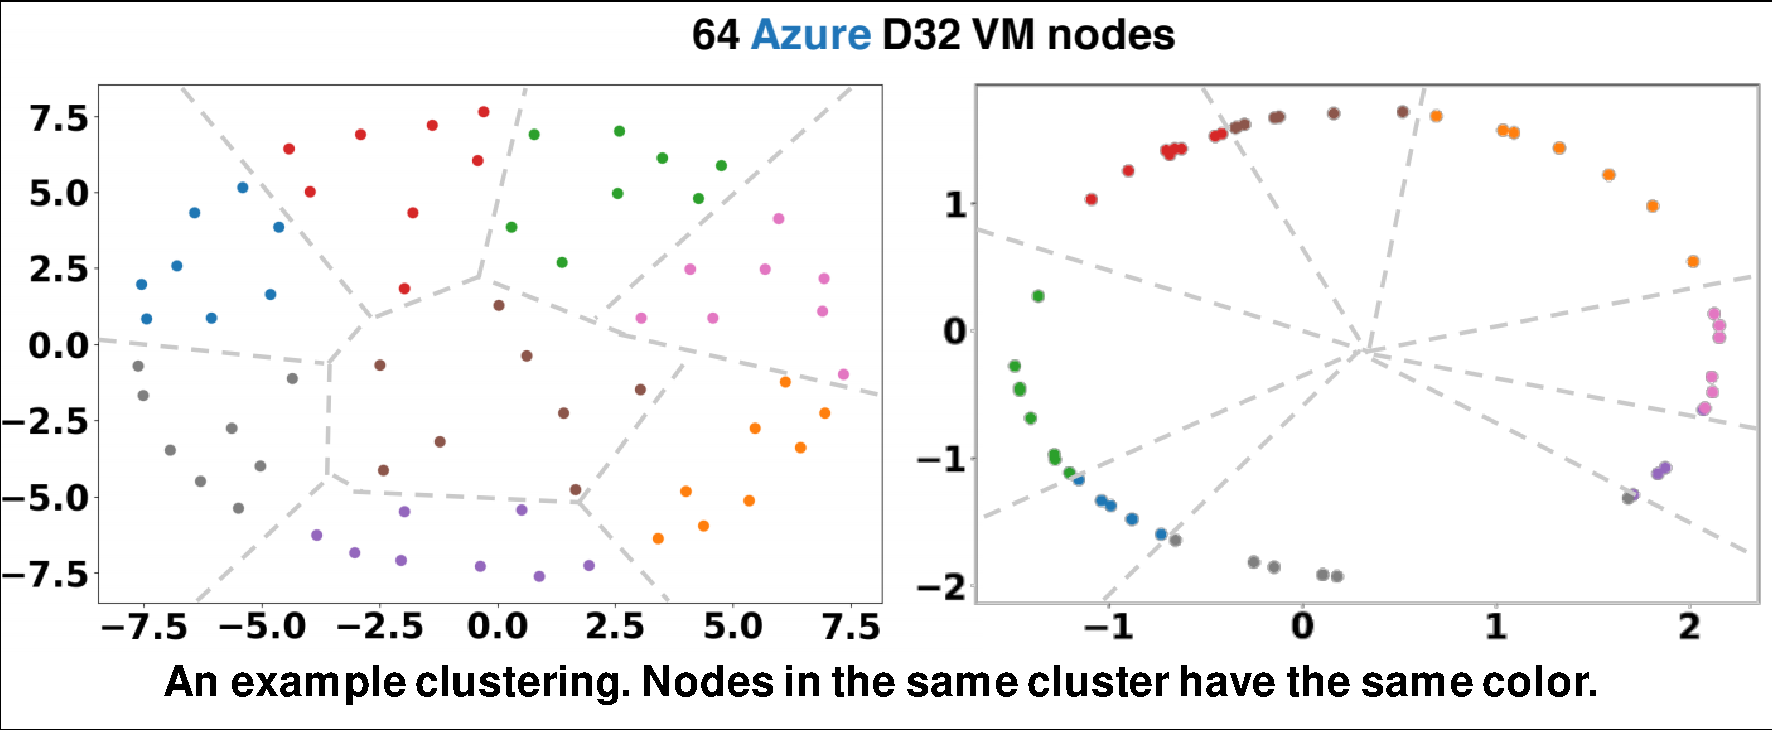
\includegraphics[width=.7\linewidth, trim= 4 4 4 4,clip]{Figures/clusters.pdf}
	\caption{Effect of $\alpha$: $\alpha = 2$ (right) generates more consistent clusters (higher AMI across 100 generated clusters) compared to $\alpha=1$ (left)} % This effectively means the resulting embedding space is more sensitive  long distances than short ones, where it is equally sensitive when $x=1$}
	\label{fig:legacy_why}
\end{figure}


%Second, consider the fact that bottlenecks will likely come from longer distances. For this reason, it can be more important to capture long distances precisely. Figure 4 demonstrates why the $x=2$ case achieves this. If we consider an error margin in capturing probe distance (which is the error we optimize here, by sum-of-squares) we can notice a key difference between $x=1$ and $x=2$. In the $x=1$ case, the error margin in euclidean space required satisfy the probe distance margin does not depend on probe distance. In the $x=2$ case however, a larger probe distance gives us a tighter error margin in Euclidean space, effectively forcing the coordinates to capture larger probe distances more precisely.

%Inspired by the Vivaldi system of \cite{dabek2004vivaldi}, we allow for "height" parameters $h_i$ for each node i. When this feature is enabled ($\mathbbm{1}_h = 1$), $h_i$ corresponds to an added, node-specific distance applied to any distance the node is involved in. We found this useful for improving the system's ability to capture ground-truth topology for some nodes (e.g. ping) but not others, which is why we allow this to be disabled.



\paragraph{Grouping Nodes for \mlha}
We now outline how \marcopolo partitions VM nodes into groups for \mlha. The goal is to generate groups that are (1) balanced, so no single group becomes a bottleneck and (2) cohesive, so VMs in the same group have good locality. We first compute the number of groups to generate, then determine the members of each group.

GMs are more likely to be the bottleneck during \mlha, as they must receive and aggregate messages at both levels. For a uniform key distribution, the following term approximates the bytes-on-wire sent or received by a GM:
\begin{equation}
   b = O\left(\frac{n}{k} + k\right)
\end{equation}
with $n$ total VMs, and $k$ groups. The GM sends and receives a message from each node within its group ($\frac{n}{k} -1$) for local aggregation, and from every other group ($k-1$) for global aggregation. This expression achieves a minimum at $k = \sqrt{n}$, giving a natural choice for group count. %., and it is empirically effective with and without them.

Once group count is selected, we use a constrained k-means clustering algorithm with k-means++ initialization~\cite{bradley2000constrained, arthur2007k} to generate balanced, locality-preserving groups. This accepts a minimum cluster size and the number of groups to generate as input. %\arvind{and number of groups also as input?} 
For perfect balance, both parameters are set to $\sqrt{n}$. %, where $k = \sqrt{n}$ in general. %, we use $k = \sqrt{n}$ (as justified in \strongrandom).

Enforcing perfect balance is not optimal in cases where VMs are naturally clustered in almost balanced but distant clusters, because in those cases some group can contain a distant member which could be assigned to a much more cohesive group with a slight imbalance, forcing an onerous bottleneck on the local aggregation step. Thus, we include a parameter, \textit{balance elasticity}, which enables a slight imbalance among clusters. We empirically found best results with values between 1.0 (perfectly balanced) and 2.0 (each group has at least $\sqrt{N}/2$ nodes). %\arvind{define the parameter -- largest/average or largest/smallest?}

%We include optional parameter $h_i$ from equation 1 which can improve the quality of embedding, but will not affect the clustering objective and can be safely ignored.

In order to evaluate the performance of \marcopolo, we also define \strongrandom, a grouping method for \mlha that operates without considering probe distances and simply produces $\sqrt{n}$ groups of size $\sqrt{n}$ uniformly at random. This is used later as a baseline.

\subsubsection{Efficient HA with \ha}
\label{sec:haimpl}
\ha transforms grouping information from \marcopolo into a hierarchical reduction plan and efficiently executes it. \ha takes the crux of \phub and applies them to a TCP context to accommodate for the cloud environment where InfiniBand is not available.
\ha supports various communication backends, including TCP, RoCE~\cite{softroce}, iWarp~\cite{softiwarp}, and InfiniBand.

%, to maintain compatibility with all environments. We now briefly describe \ha in the context of TCP. %On clouds with Ethernet-only support such as EC2, \ha can still support RDMA with SoftiWarp~\cite{softiwarp} and SoftRoCE~\cite{softroce}, although we didn't find any performance benefit of doing so compared to using a native TCP backend.

\paragraph{Generating an Aggregation Plan}
\label{sec:generatingAggregationPlan}
\ha chunks buffers into 64KB segments for better load-balancing across processor cores and overlapping of the transmission of gradients with aggregation. % but at the cost of potentially more packets. \ha uses chunk size of 64KB. % for TCP and 8KB for RDMA.

%identifying the buffers and their sizes to aggregate. \ha first creates chunks of buffers. Chunks are important if the supplied buffers have various sizes and are hard to balance the load. \ha prefers smaller buffer chunks because they allow for more fine-grained overlapping of data transmission and aggregation, as each chunk can be aggregated independently to take advantage of the fact that aggregation is an element-wise operation. However, a chunk size too small is harmful as they may not saturate the network and requires excessive computation overhead: generally, we find chunk size between the network MTU size (generally 1.5-9KB) and a few hundreds of KBs to be optimal depending on the workload and environment.

%Generally, once \ha has a list of chunks with roughly the same size, it finds each chunk a \textit{local master (LM)} for each clustered group of nodes. LMs take care of leaf-level aggregation of a chunk using central aggregation. \ha then assign one of the LMs as \textit{global master (GM)}, so that LMs only send per-group aggregated chunk to GM, by going through the four steps described in \ref{sec:2lhaOverview}. %Small buffers are treated differently, however: if buffers are small, the time to traverse an additional two hops (with \mlha) may not be compensated by the reduced cross rack traffic. It is better to ignore the cluster topology and treats the network as flat. \ha uses a flat topology for buffer $b$ if $lat(GM(b),LM(b)) \approx \frac{SIZE(b)}{bw(GM(b), LM(b))}$, which means the propagation latency is comparable to transmission delay. Note we use the full bandwidth as an overestimation for this purpose, because in reality the bandwidth is shared by multiple flows. This rule is usually applied to buffers of sizes of tens or hundreds of bytes. 


Since \ha is bottlenecked by the slowest inter-group transfer, which in turn is bottlenecked by the slowest intra-group transfer, \ha assigns chunk GMs and LMs such that each group (or node) has a number of GMs (or LMs) proportional to its cardinality. \ha uses an approximation set partition algorithm to achieve this. %Assignment of LM placements in each group follows a similar fashion. 
%as the aggregate available bandwidth scales with the size of a group. % Now consider the min-cut of the bandwidth for each cross rack link in the inferred cluster. The value of the bandwidth min-cut is proportional to the cardinality of the cluster.%., until it reaches the bandwidth of a physical uplink ($B_{upward}$) from ToR to the network core. % This value is currently a changeable parameter ($B_{upward}$) in \ha. 
%Since aggregation latency is determined by the slowest group, \ha need to balance GM assignments cross racks: more GMs should be placed in larger groups.
%but up to a point. 
 %assign GLMs to different clusters based on the min-cut value. The bandwidth min-cut for each group is estimated as the less of $B_{upward}$ and $|C| * B_{vm}$.


%The same argument goes for RLM placements in each rack. \ha uses a similar mechanism to assign RLMs. This is simpler than assigning GLMs because the min-cut bandwidth of each node is equal to the bandwidth provisioned by the cloud, usually 10Gbps. Since a single TCP connection may not be able to saturate a 10Gbps link (as some cloud limits the bandwidth of a single flow~\cite{Placemen48:online}), during communication, \ha establishes multiple connections to each peer and the total transferred data is load-balanced across all connections.

\ha then generates a schedule that executes the steps in \textsection \ref{sec:2lhaOverview} for each chunk. A schedule consists of a set of chunk-action pairs, where action is one of the following\footnote{With these action primitives, \ha can support arbitrary reduction graphs.}:
\begin{itemize}[noitemsep,topsep=0pt,parsep=0pt,partopsep=0pt]
    \item \textbf{SendTo(nids)}: send the content in the current \textit{merge buffer} to the list of nodes specified in \textit{nids}. SendTo is a non-blocking operation, and its status is inferred by whether subsequently anticipated data is received.
    %\item \textbf{ReceiveFrom(nids)}: receive the content in the merge buffer of \textit{nids}. ReceiveFrom is a blocking operation, and it finishes when all updates are received.
    \item \textbf{ReceiveFrom(nids)}: block until the chunks from \textit{nids} are received and aggregated into the merge buffer.
    \item \textbf{Fetch}: notifies \ha that a framework-supplied buffer is ready to be processed.%a fetch action is taken when the calling framework notifies \ha that a buffer can be read. %Depending on the framework, \ha may create a copy of this buffer in case it is modified during aggregation.
    \item \textbf{Deliver}: writes the content in the merge buffer back to the framework-supplied buffer. %\arvind{Deliver instead of Delivery?}
\end{itemize}

A schedule is represented as a DAG where dependencies are edges and nodes are primitives, avoiding false dependencies between local and global aggregation.

\paragraph{Executing an Aggregation Schedule}
\label{sec:2lhae}

%When a job starts, \ha creates two merge buffers for each chunk (details below) and one receive buffer for each peer. %Merge buffers are padded to the nearest cache-line size for efficient reduction using SSE or AVX. 
\ha first performs rendezvous with an out-of-band mechanism (e.g., Redis), establishing multiple connections per pair of VM as cloud providers can restrict per-stream bandwidth~\cite{Placemen48:online}. \ha preserves intra-node locality by maintaining a load-balanced map from a chunk to a connection, and then by further associating the connection to a particular processor core~\cite{Pesterev:2012:INC:2168836.2168870}.

%\ha then connects the mesh prescribed by the schedule. For TCP connections, \ha maintains two flows per network device per remote node to saturate bandwidth; for RDMA-based backends, \ha maintains one connection per network device per remote node (\ha can always materialize additional virtual interfaces as needed). The rendezvous of addresses (IP ports and QP numbers) and memory regions are performed using a central redis server. 

%\begin{figure}
%	\centering
%	\includegraphics[width=\linewidth, trim=0.5 0 0 3,clip]{Figures/2lhae.pdf}
%	\caption{\ha preserves locality by associating a chunk with a particular core and a connection.} % This effectively means the resulting embedding space is more sensitive  long distances than short ones, where it is equally sensitive when $x=1$}
%	\label{fig:2lhae}
%\end{figure}

 %(Figure~\ref{fig:2lhae}).

%\ha groups connections by underlying network device. Each device is then associated with one poll descriptor. Each poll descriptor is further tied to a particular processor core, promoting locality~\cite{Pesterev:2012:INC:2168836.2168870}. The buffers that need communication are load-balanced across network devices first, then load-balanced again across connections.

%\ha spawns worker threads to execute a routine event loop. The event loop pulls data in/pushes data out from/to connection, and polls data from \textit{ready queue}, and \textit{defer queue}.

We now focus on how \ha efficiently supports the four actions, hiding communication latency and avoiding excessive synchronization.

When a framework calls \code{reduce(chunk)}, \ha retrieves the thread ID, suspends it, and enqueues \code{chunk} to the ready queue. Its worker threads poll the ready queue to retrieve \code{chunk} and transition the buffer into the Fetch state, copying gradients from the supplied address, then set the state of buffer to SendTo. %If multiple buffers are available, \ha prioritizes the buffer that corresponds to the later layers of the neural network, because they are required first during backward propagation. When fetch of a buffer is done, \ha transfers the buffer state to the next step specified by the schedule, SendTo. 

SendTo is an asynchronous operation that simply enqueues data to a send FIFO queue. A cursor is used for each TCP connection if a send operation cannot finish. \ha enforces that the order of bytes on the wire corresponds exactly to the order in which SendTos are issued. This saves metadata overhead as only a 4B integer per flow that encodes the chunk ID is required.
% Avoiding mixed transfers of different chunks for a single network flow lets \ha minimize metadata overhead, as only a 4B integer that encodes the chunk ID is required. %For RDMA connections, we use immediate field of a \code{ibv\_wr} to encode metadata and choose \code{IBV\_WR\_RDMA\_WRITE\_WITH\_IMM}.


SendTo is followed by ReceiveFrom. \ha allows streaming aggregation for each buffer in ReceiveFrom state to a \textit{merge buffer}. A counter is incremented when a chunk is fully received from a peer, and when the counter reaches the target, this step concludes. \ha transitions current buffer state to SendTo or Deliver based on schedule. 
%the \ha worker thread aggregates that chunk to the current merge buffer (aggregation can start at a single floating point granularity, but \ha uses SSE or AVX to aggregate whenever possible). A counter associated with a merge buffer is then incremented. 
%When the counter reaches the expected number, ReceiveFrom for that buffer is finished, and the schedule transitions into the next step, which can be another SendTo, or Delivery.


The last step of a schedule is Deliver, where \ha copies the final value to the framework-supplied address. \ha then wakes up the thread that called \code{reduce}. \ha alternates between two merge buffers per chunk for synchronous training to overlap local computation on a chunk with transfers of that chunk to peer nodes.
%Since \ha cannot immediately reuse the merge buffer from last iteration, as the transfer to peer nodes may not finish. \ha alternates two merge buffers per chunk for synchronous training because the peers lag behind at most one iteration. %The flipping step is required because SendTo is asynchronous and can finish before data is on the wire. 
%If the training framework calls \code{reduce} again, the newly-fetched data will overwrite the original merge buffer. 


%Note that the framework does not call another \code{reduce} with the same \code{bufferID} when one is active. Since it is certain when iteration $i+1$ finishes, all merge buffers for all keys of iteration $i$ would have already been sent out (otherwise if remote peers did not receive buffers for iteration $i$, they would not participate in finishing iteration $i+1$ in the first place!). By taking advantage of training is synchronous, we can use two merge buffers to avoid waiting for a SendTo completion signal.

%Not all nodes proceed at the same speed as slower nodes may see incoming data from faster nodes without having the buffer state in ReceiveFrom. In this case, \ha eagerly accepts the data in the receive buffer, without touching the merge buffer because it may be overwritten by a late \code{reduce} call. \ha bookmarks the incoming chunk ID to a deferred queue, which is polled frequently to check if any progress can be made. 
%Saving data to the receive buffer when not in ReceiveFrom state is safe, because each peer only sends one copy of data for each chunk. 

%because \ha is sure that a buffer is sent exactly once per iteration. For bookkeeping, \ha maintains a deferred queue, which is queried later. 



%\subsubsection{Changing an Aggregation Schedule}
%\label{sec:changingPlan}
%\ha dynamically swaps in new aggregation plans to react to network changes by reassigning LMs and GMs. This can be implemented efficiently as coherence is optional in DL~\cite{recht2011hogwild, Wei:2015:MCC:2806777.2806778,BSP,SSP,Litz,orpheus}.% shows it is not required to achieve high accuracy. %\ha can get away by taking advantage that learning itself is a stochastic process: by maintaining a keeping a strongly coherent view of model during normal operation and a bounded-staled, relaxed view of model during change of aggregation schedule, which is known to not affect accuracy

%Schedule changes start by blocking subsequent calls to \code{reduce}. \ha then attempts to bring its polling threads to a safe point, %so that aggregation schedule for all buffers can be reset to Fetch stage. A safe point is 
%which is reached by first draining the send queue then transitioning the buffer state to Fetch. %, avoiding transferring old data when a new schedule is installed.\
%Each buffer is then given a 5s timeout to do so, and after which \ha signals its peers that it is ready to switch to a new schedule for that chunk. \ha recovers chunks that are affected by requeueing them to the ready queue. 

%\ha supports a transparent process for switching to a new aggregation schedule, with the end result being that chunks whose reductions are interrupted by schedule changes may hold values from the previous iteration, while chunks whose reductions are uninterrupted reflect the new values of the current iteration.

\begin{table}[t]
	\centering
	\small
	%\footnotesize
	\begin{tabular}{|c|c|}
		\hline 
		Property & \ha Optimization \\
		%\hline
		%Wide range of buffer sizes & Size-based agg. route selection. \\
		\hline
		Fixed comm. pattern & No explicit acknowledgement \\
		\hline
		Fixed buffer size & Minimal metadata \\
		%\hline
		%Later layer depended on first & Prioritize later layers \\
		\hline
		One reduction per layer & Only 2 merge buffers per layer; \\
		       per iteration    & Eagerly accepts chunks \\
		\hline
		Training is stochastic & Switching plans quickly and cheaply \\ 
		\hline
		
	\end{tabular}
	\caption{Codesigning \ha with training workload.}
	\label{table:codesign2lha}
\end{table}

Table \ref{table:codesign2lha} summarizes how \ha is designed to take advantage of properties in the distributed training workload to lower its overhead.

\subsubsection{Reacting to Network Changes with \autoplink}
\label{sec:autoplinkimpl}
\autoplink collects performance information from \ha and watches for sudden changes in link conditions, reflected by the current training speed. %Instead of running \marcopolo in the background, which itself is resource intensive, \plink needs to take a lightweight approach that directly pinpoints the link bottleneck of training. 
The goal of \autoplink is to dynamically compensate for link changes by redistributing LMs and GMs to VMs, so the time to finish an iteration is similar at both local and global levels.  %that slower VM nodes are serving less as GM or LM of chunks. %, so that nodes with less bandwidth are assigned fewer chunks. 

A perfect initial LM and GM assignment is hard, even if we have bandwidth probe measurements. Consider an aggregation plan $S$, where the \textit{effective bandwidth} of node $i$ to $j$ while running aggregation $S$ is $BW(i,j)$.  Clearly, finding the best $S$ analytically relies on $BW(i,j)$ to be precisely measured or modeled, but $BW(i,j)$ has a circular dependency on $S$ itself. \autoplink thus makes approximations when optimizing the assignments. %, because it depends on the actual transfers dictated by $S$. %Meanwhile, $BW(i,j)$ might change due to competing traffic. To counteract this effect, the number of bytes transferred from $i$ to $j$ according to $S$, denoted by $D(i,j)$, should also reflect the change. Moreover, the time to compute model updates in different VM nodes may also differ, creating the straggler effect and adding to the complexity. 

%\autoplink cannot simply minimizes each link's individual transfer time, because they all share the bandwidth of a given node, nor can it minimize the maximum transfer time, because $D(i,j)$ constitutes the total transfers for all different stages $p$ in 2LHA, and thus may not overlap with other transfers. 
At a high level, \autoplink works in two phases: (1) a \textit{Quicktune} phase where a one-shot, global adjustment of GM and LM assignments is done to adapt to the network change immediately; and (2) a \textit{Finetune} phase where \autoplink uses a performance model to find the current performance bottleneck in the system, and moves GMs and LMs away from it in a stepwise, increasingly aggressive manner.

\paragraph{Quicktune}
Quicktune aims to minimize the maximum transfer time of each node. Quicktune can be best summarized formally as follows: let $GM(i,c) \in \{0,1\}$ and $LM(i,c) \in \{0,1\}$ be the boolean variables to be solved, which indicate whether node $i$ is the GM or LM of chunk $c$. Let $G(i)$ be the group of node $i$, $|G|$ the number of groups and $S(c)$ the size of $c$ in bytes. Our goal is to:

minimize
\begin{align*}
\small
\label{eq:quicktuneobj}
   \quad max(t_i = \frac{\sum_{c}S(c)(LM(i,c)|G(i)| + GM(i,c)|G|)}{\sum_{n}BW(i,n)})
\end{align*}

subject to
\begin{align*}
\small
    \forall_{i,c} \quad GM(i,c) = 1 \implies LM(i,c) = 1 \\
    \forall_{c} \quad \sum_{i}GM(i, c) = 1 \\
    \forall_{c,g \in G} \quad \sum_{i \in G(g)}LM(i,c) = 1
\end{align*}

Quicktune solves this with an approximation: it first distributes GMs to different groups, with the number of GMs assigned to each group proportional to the group aggregate bandwidth $\sum_{m \in G(i)}\sum_{n \notin G(g)}BW(m,n)$, then distributes LMs inside each group to different members in a similar fashion, using aggregate per node bandwidth.

%This is effective because groups are balanced in \plink \mlha schedules, and there are many more chunks than there are nodes, practically making every node a GM of a certain chunk, so the effect of being a GM in each group can be ignored. 

%To retrieve $BW(i,j)$, \autoplink queries per connection stats directly from the OS~\cite{NetlinkW13:online, mathis2003web100}.% Since this bandwidth is an average reading, \autoplink filters by the \code{app\_limited} field: bandwidth measured only when the outbound throughput is not throttled by the sending application is recorded. To further reduce averaging effects, \autoplink queries this after each successful \code{write} call.

\paragraph{Finetune}
Quicktune is limited as it assumes constant effective bandwidth across different schedules and ignores node balance. Finetune, however, amends this by gradually \textit{evolving the current schedule}, using both the currently measured $D(i,j)$ and $B(i,j)$ to pinpoint the current bottleneck node in the system, and then moves away its load while maintaining balance based on \textit{blame}. Blame for node $i$ ($B(i)$) has two major weighted parts: \textit{time} $t(i)$ and \textit{imbalance} $l(i)$. \autoplink collects per connection stats including link $RTT(i,j)$, bandwidth $BW(i,j)$ through the OS~\cite{NetlinkW13:online, mathis2003web100}, and computes $t(i)=max_{j}RTT(i,j) + \frac{\sum_{j}D(i,j)}{\sum_jBW(i,j)}$ and normalized $\hat{t(i)} = \frac{t(i)}{mean_n t(n)}$. %Note that we use a first order model to predict reduction time, instead of measuring it directly, because actual reduction time includes overheads from other nodes and we shouldn't blame those on node $i$.%
Further, we let $l(i) = \sum_j{D(i,j)}$ and weighted $\hat{l(i)} = \frac{l(i) -  min_nl(n)}{max_nl(n) - min_nl(n)}$. Finally, blame is defined as $\beta \hat{l(i)} + \gamma \hat{t(i)}$.%(empirically, $\beta=1,\gamma=5$).  %Note how $D(i,j)$ is simply read from the previous schedule in Finetune, a core difference to Quicktune.

With blame for each node available, Finetune attempts a move of a single GM (or if not available, an LM) from the node with highest blame to the lowest, if $\frac{max_iB(i)}{min_iB(i)} >\epsilon$ (a configuration parameter). If Finetune repeatedly identifies the same bottleneck node, it moves exponentially more LMs and GMs in each step. %The number to move is reset to 1 if the bottleneck changes.


%Finetune's metrics are directly inspired by those used in profiling concurrent systems, notably~\cite{Anderson:1990:QTT:98460.98518,AUDIT}, which distributes blames to active tasks (root cause) sharing the resource, and focuses on first order effects~\cite{80132,211299} (most blamed nodes first). 

\autoplink uses a central daemon to collect performance metrics and generate new schedules, and is triggered by a sudden change (e.g., larger than 20\%) in training performance. \autoplink signals \ha to install the new schedule. %, which then proceeds with the steps in \textsection\ref{sec:changingPlan}. % to start using the new schedule.

%\arvind{some comments: (1) this overall sounds very heuristicy and will likely make the reviewers complain - the less heuristicy it is, it would be better; (2) not clear we need to describe both quicktune and finetune - might be simpler to just describe finetune; that might help it sound less heuristicy; (3) try to be as precise as possible about the algo.}

\subsubsection{Integration with Training Frameworks}
\label{sec:integration}
Integrating \plink with a training framework is straightforward. \plink{}'s initialization requires only a list of nodes and buffer sizes/addresses from the training framework. %Reduction is done by calling \code{reduce} in appropriate places.
Here we demonstrate how \plink can be integrated with systems with training frameworks that have different design decisions.

Caffe2/Pytorch uses blocking reduction. \plink integration is done by extending Gloo~\cite{facebook35:online}'s \code{algorithm} object. Caffe2/Pytorch, by default, uses a concurrency limit to control the number of established connections per peer and simultaneous \code{allreduce} calls. \plink instead uses a single \ha instance to multiplex all requests.

MxNet uses an asynchronous callback pattern, but \plink{}'s \code{reduce} is blocking. A separate thread is launched for invoking callbacks through \code{kv\_apps}'s infrastructure when a chunk has finished. Support for MxNet is enabled by extending PSLite~\cite{dmlcpsli50:online}'s \code{van} object. %Initialization of \plink is done by hooking into the \code{init} call of \code{kv\_dist\_server}.

